% Chapter 5

\chapter[E-Puck Robot Platform]{E-Puck Robot Platform} % Main chapter title

\label{Chapter5} % For referencing the chapter elsewhere, use \ref{Chapter1} 

%----------------------------------------------------------------------------------------

\section{Overview}
The e-puck robotic platform, created by a team at the \textit{Ecole Polytechnique Fédérale de Lausanne} \cite{epuck}, is a small, relatively inexpensive, multi-purpose robotic platform designed for for education and research pursuits regarding robotics and multi-robot systems. The platform is widely used in swarm robotics research, featuring in a number of publications. The e-puck was chosen as the first target platform for this system for a number of reasons. Firstly this was one of the platforms available in suitable numbers in the York Robotics Laboratory (YRL) at the University of York, where the practical work for this project was carried out. Secondly the platform's wide use in swarm robotics research helps to show the broad applicability of the system, and better demonstrates its value when compared to a less widely used or bespoke platform. Finally the platform's extensible design meant that it could be equipped with a Linux extension board, a configuration frequently used at the YRL. This made the use of WiFi for wireless data transfer feasible, and was a large part of the reason for the e-pucks choice. This section provides details of the e-puck robot's hardware, including processor, sensors and actuators, as well as details of the configuration used for this project, including the Linux extension board. Figure \ref{fig:EPuck} shows the e-puck robot [TAKE NEW PICTURE].

\begin{figure}
	\begin{center}
	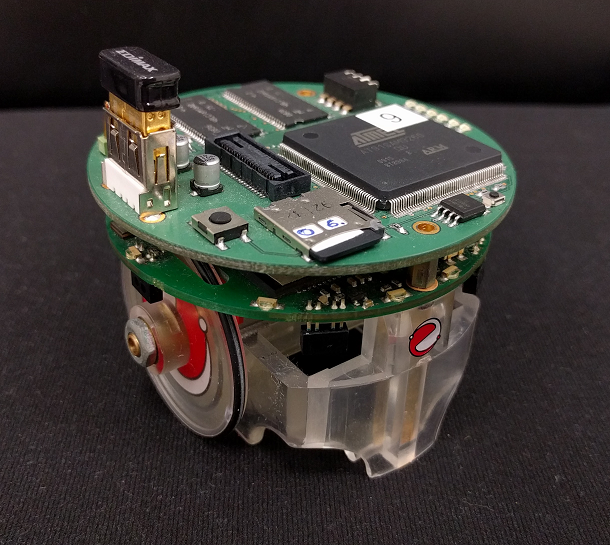
\includegraphics[scale=0.6]{EPuck.png}
	\decoRule
	\caption[The e-puck Robot]{The e-puck robot.}
	\label{fig:EPuck}
	\end{center}
\end{figure}

%----------------------------------------------------------------------------------------

\section{Processor}
The e-puck features a dsPIC 30F6014A microprocessor, designed and manufactured by Microchip Technology Inc. This is a general purpose 16-bit CPU, with relatively low performance by modern standards. The processor features 68 I/O pins, which are connected to the e-pucks various peripherals. Due to the use of the more powerful Linux extension board discussed in section \ref{LinuxExtensionBoard}, the primary use of the PIC processor in the e-puck configuration for this project is to interface with the e-puck's hardware. This involves receiving commands from the Linux extension board and sending appropriate control signals to the robot's actuators, as well as reading the robot's sensors and passing the retrieved sensor data back to the Linux extension board.

\subsection{Firmware}
Prior to the start of this project the YRL had already developed a library of low level code allowing the PIC to function in the hardware interface role as described above, controlled through the UART serial port. This firmware code was used as-is on the e-puck PIC controllers throughout the project.

%----------------------------------------------------------------------------------------

\section{Actuators}
The e-puck robot features two wheels, independently actuated by two step motors. The wheels have a diameter of approximately 41mm. The motors can rotate the wheels at an approximate maximum speed of 1000 steps per second in either direction, where 1000 steps is one full revolution. The robot also features a ring of 8 red LEDs around the edge of the main circuit board. 

%----------------------------------------------------------------------------------------

\section{Sensors}
The e-puck robot features a number of different sensor sets, of which only some are used in this project. A set of 8 IR proximity sensors are arranged around the circumference of the robot, with four positioned on the forward hemisphere, two positioned at right angles to the forward direction (one on either side) and two more positioned on the backward hemisphere at roughly 45 degrees either side of the backward direction. Figure \ref{fig:EPuckIRSensors} shows this layout. The IR sensors can be used in two modes - active and passive. In active mode the sensor emits an IR pulse and measures the IR strength of the reflection, whereas in passive mode the sensor simply samples the IR strength without emitting a pulse. The passive mode can therefore be used to get a 'background' IR reading, which can be compared to the active reading to improve accuracy. The IR sensor is of particular interest to this project as it is a frequently used tool when working with robots, especially robot swarms.

\begin{figure}
	\begin{center}
	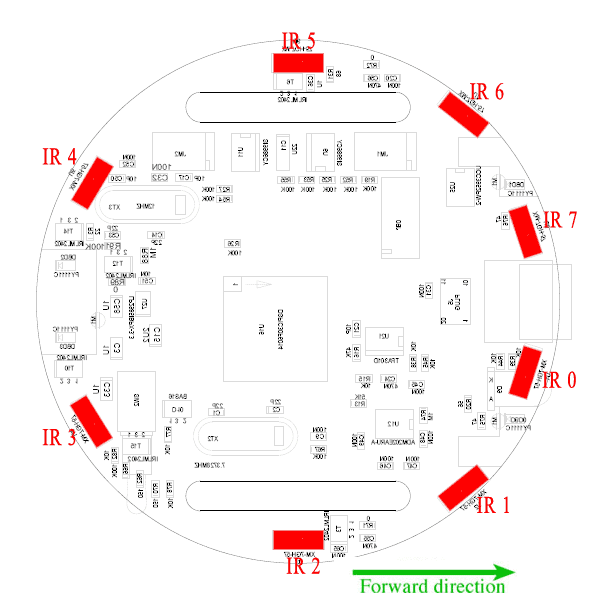
\includegraphics[scale=0.4]{EPuckIRSensors.png}
	\decoRule
	\caption[e-puck IR Sensor Layout]{The layout of the IR sensors on the e-puck robot.}
	\label{fig:EPuckIRSensors}
	\end{center}
\end{figure}

The robot also features three microphones, a 3 axis accelerometer and a camera. Due to the bandwidth required to use the microphones and camera they were considered a low priority for this project. [ACCELEROMETER?] 

%----------------------------------------------------------------------------------------

\section{Linux Extension Board} \label{LinuxExtensionBoard}
For this project the e-pucks were fitted with an extension board featuring a 32-bit ARM9 processor running a modified Linux operating system \cite{LinuxExtensionBoard}, developed by Wenguo Liu, and Alan F.T. Winfield. In this configuration the ARM processor, an Atmel AT91, takes charge of the high level robot control logic, as well as any intensive data processing operations. The dsPIC processor is then used to control the low level actuator and sensor control, running in parallel with the ARM processor and communicating via UART. The extension board provides a USB port, and for this project a WiFi adapter was connected to each robot. The controller code running on each robot could then make use of the standard IP network layer protocol, and the standard transport protocols TCP and UDP.

%----------------------------------------------------------------------------------------
